\documentclass[a4paper,11pt,openany,extrafontsizes,oneside,article,twocolumn]{memoir}

%%\directlua{pdf.setminorversion(3)}

\usepackage{fontspec}

\setmainfont[Numbers=OldStyle]{Linux Libertine O}
\setsansfont[Numbers=OldStyle]{Linux Biolinum O}
% \setmonofont{Inconsolata}
\setmonofont[Scale=0.83]{Bitstream Vera Sans Mono}
% \usepackage{lmodern}

\usepackage{polyglossia}
\setdefaultlanguage{english}

\usepackage{graphicx}
\usepackage{xcolor}
%\usepackage{wrapfig}
\usepackage{subcaption}
%\usepackage{lettrine}
%\usepackage{tikz}
\usepackage{amsmath,amssymb}
\usepackage{booktabs}

% \usepackage{unicode-math}
% \setmathfont{texgyrepagella-math.otf}

%\usepackage{pdfpages}

\usepackage{microtype}

%% Propriétés du document PDF
\usepackage[unicode,colorlinks=true,linkcolor=blue]{hyperref}

\hypersetup{
  pdfauthor={P272},
  pdftitle={Statistical Machine Learning: Assessed Practical},
  pdfsubject={Assessed Practical},
  pdfkeywords={stats,practical,report},
  pdfpagemode=UseOutlines,
  pdfpagelayout=TwoColumnRight
}

\renewcommand{\chapterautorefname}{section}

\definecolor{bg}{rgb}{0.95,0.95,0.95}

\usepackage{minted}
\setminted[r]{autogobble,fontsize=\footnotesize}

%% Pour la classe memoir /!\

%% Marges
\setulmarginsandblock{3cm}{3cm}{*}
\setlrmarginsandblock{3cm}{3cm}{*}
\checkandfixthelayout%

%% Numérotation des divisions logiques
\setsecnumdepth{subsection}
\maxsecnumdepth{subsection}

%% Profondeur de la ToC
\settocdepth{subsection}
\maxtocdepth{subsection}

%% Style des titres des divisions logiques
\setsecheadstyle{\sffamily\Large\scshape}
\setsubsecheadstyle{\sffamily\large\scshape}

%% style des environnements description
%\renewcommand*{\descriptionlabel}[1]{\hspace\labelsep
%  \normalfont\itshape #1}

%% épigraphes
%\setlength{\epigraphwidth}{0.5\textwidth}
%\epigraphtextposition{flushleftright}


\author{\sffamily\LARGE P244\and\LARGE P272\and\LARGE Pxxx}
\date{\sffamily Week 8, Hilary Term 2018}
\title{\sffamily\scshape\HUGE Statistical Machine Learning\\[.2em]
\LARGE Assessed Practical}



%%% Local Variables:
%%% mode: latex
%%% TeX-master: "report"
%%% End:


\clubpenalty=10000
\widowpenalty=10000
\raggedbottom%

\newcommand{\rsq}{R$^2$~}
\newcommand{\betac}{\widehat{\beta}}
\newcommand{\lkh}{\widehat{L}}
\newcommand{\loglkh}{\ln(\widehat{L})}
\newcommand{\ypred}{\widehat{Y}}
\newcommand{\eg}{\textit{e.g.~}}
\newcommand{\expectation}[1]{\mathbb{E}[#1]}
\newcommand{\var}[1]{Var[#1]}
\newcommand{\RP}{\textcolor{red}{\large{\textbf{TBC~}}}}
\newcommand{\fbf}{\texttt{BF}}
\newcommand{\yTrue}{y}
\newcommand{\yPred}{\hat{y}}
\newcommand{\ri}{\rho_i}
\newcommand{\rit}{\rho_{i,t}}
\newcommand{\muit}{\mu_{i,t}}
\newcommand{\thtk}{\widetilde{\theta_k}}
\newcommand{\fhome}{\texttt{Home}}
\newcommand{\fpos}{\texttt{Pos}}
\newcommand{\sq}{$^{\text{2}}$}

%% Style de chapitre
%\chapterstyle{}
\setlength{\beforechapskip}{30pt}
\renewcommand{\chapnamefont}{\sffamily\LARGE\scshape}
\renewcommand{\chapnumfont}{\sffamily\LARGE\scshape}
\renewcommand{\chaptitlefont}{\sffamily\LARGE\scshape}

\tightlists%


\begin{document}

\twocolumn[
\maketitle

\begin{onecolabstract}
  In this report, we consider the problem of determining the gender of
  an individual in a picture. More precisely, using a set of features
  derived from the original images, we try to fit a machine learning
  model that can accurately classify individuals as male and female,
  and represent its confidence in the classification.

  The performance of the model was evaluated through a Kaggle
  competition, in which we submitted predictions as team ``The Poisson
  Fishermen''.
\end{onecolabstract}

\tableofcontents*
\newpage
]



\chapter{The data}

\section{Exploratory Data Analysis}

The data available are pre-processed data from male and female
pictures. Each picture is represented by a 128-numbers long vector of
features and a label: 0 for male, 1 for female.

The labelled training set is composed of 15 000 observations, about
half of which are of female individuals. The recorded features are all
roughly centred and have standard deviations close to 0.9.

The exploratory data analysis does not show any feature particularly
standing out. After a PCA, even the first principal component carries
only around 3\% of the total variance, which suggests variability is
widespread across features. Likewise, the Spearman correlations
between individual features and the labels are rather low (all between
-0.3 and 0.3 with most much closer to 0).

Despite this lack of interpretability of the features, the data shows
good separability. A simple logistic regression gives 92\% accuracy
when predicting the labels. Likewise, using T-SNE (t-distributed
stochastic neighbour embedding), an unsupervised method that give a 2D
representation of the dataset, clearly separates most males and
females (\autoref{fig.tsne}). This is promising for the task at hand,
since it means that separation of males and females is quite feasible.

\begin{figure}[h]
  \centering
  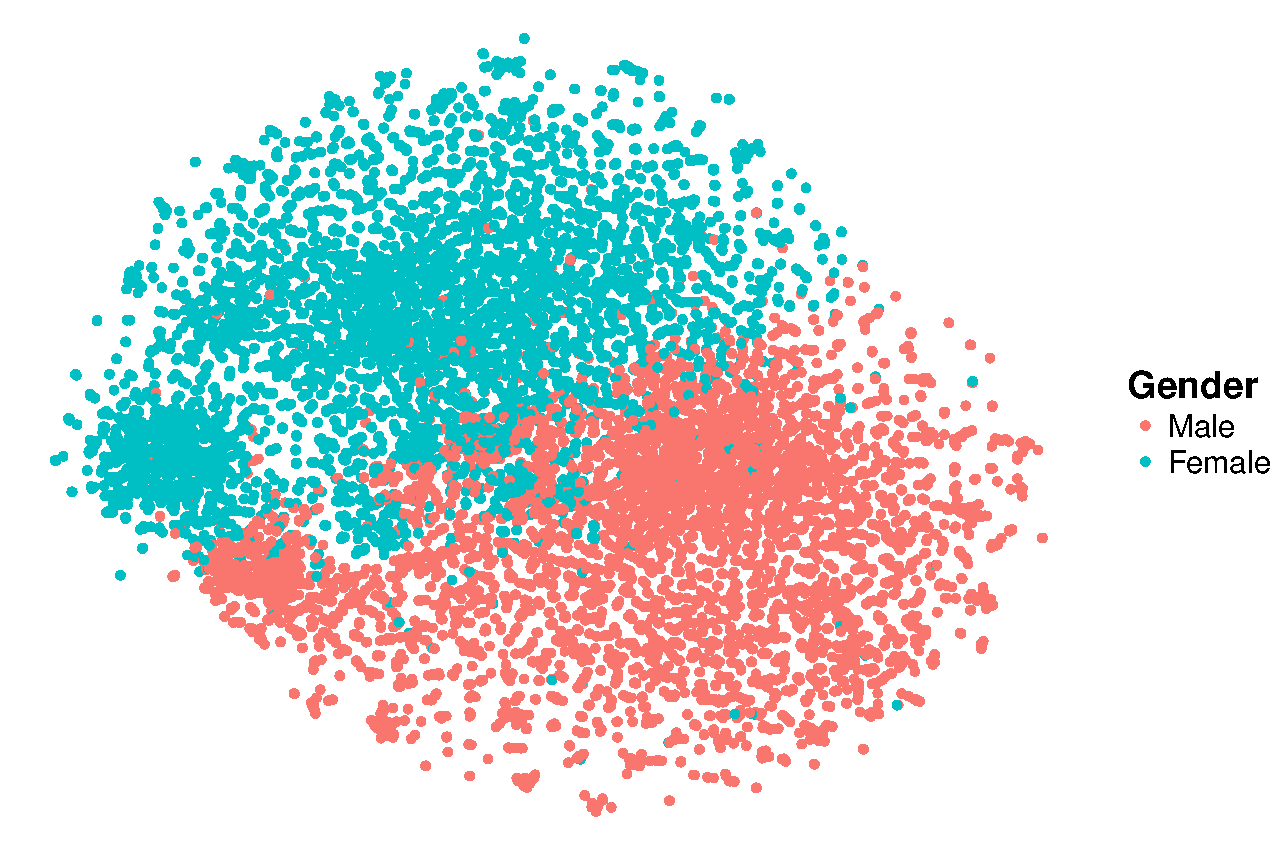
\includegraphics[scale=0.3]{tsne.pdf}
  \caption{Unsupervised 2-dimensional embedding of the data}%
  \label{fig.tsne}
\end{figure}

\section{Evaluating of the model}

To evaluate the performances of our models, the log loss, aka logistic
loss or cross-entropy loss, is used:
\[ -\log(\yTrue | \yPred) = -(\yTrue \log(\yPred) + (1 - \yTrue)
  \log(1 - \yPred))\] with $y$ the true label and $\hat{y}$ the
predicted one. A particularity of this loss is that high confidence in
a wrong prediction is very heavily penalized. This means that not only
classification should be accurate, but predictions must also be
conservative when there is some doubt on the label.

\begin{figure}[h]
  \centering
  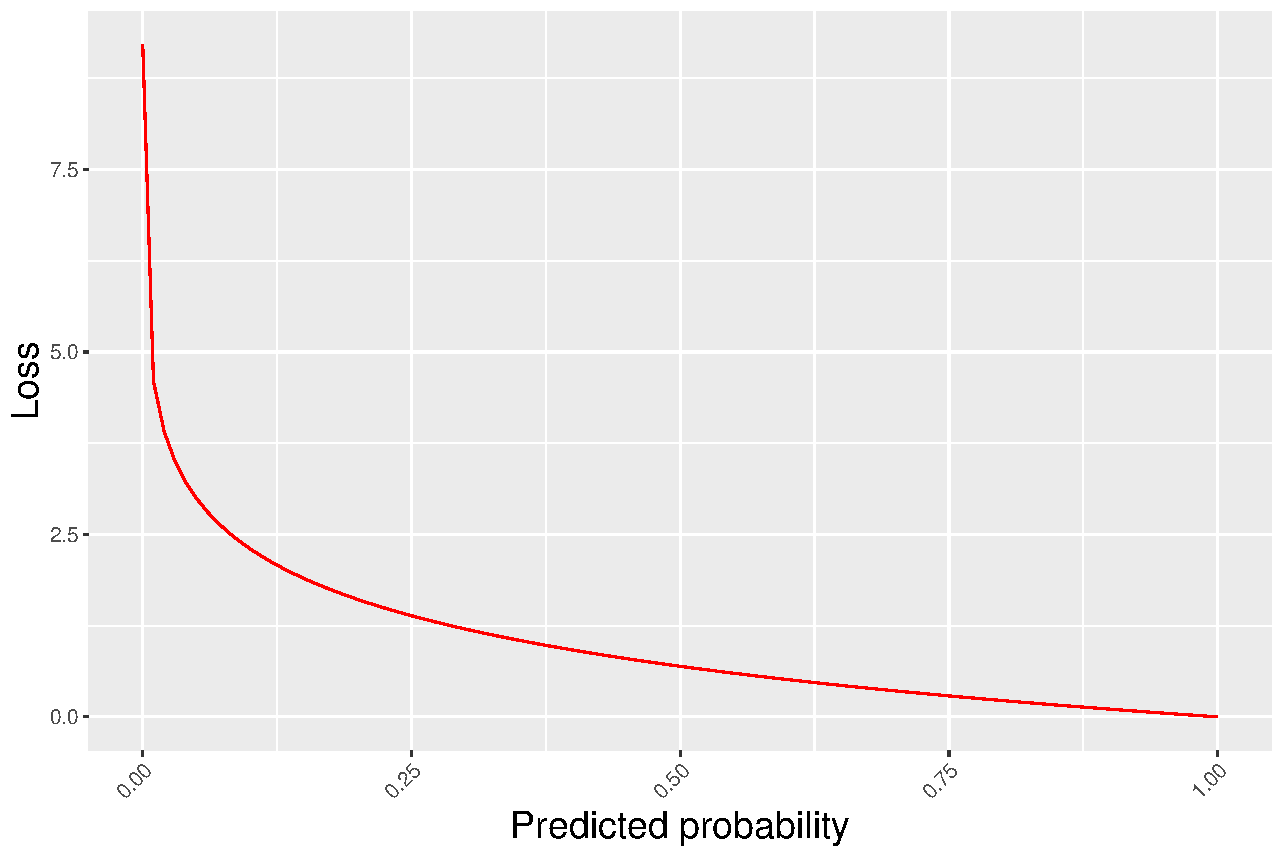
\includegraphics[scale=0.3]{loss.pdf}
  \caption{Log loss when the true label is 1}%
  \label{fig.loss}
\end{figure}

\chapter{Building the model}

\section{Basic classifiers}

Given the good separability of the data, we started by experimenting
with very simple algorithms. Our first successful attempt was the
Quadratic Discriminant Analysis (QDA), which both ran almost
instantaneously and yielded an accuracy over 98\%. $k$-nearest
neighbours ($k$-nn) with 10 neighbours had similar precision.

However, in both cases the log loss remained higher than even the
simple logistic regression (even though its classification accuracy
was lower). This is because the previous algorithms are not
well-calibrated: the exact value that they give when predicting a
probability is not representative of their true classification
performance. This causes them to be over- or under-confident in their
probability estimates, and they are thus heavily penalized by the log
loss metric. Although some methods exist to calibrate such algorithms
(using an isotonic regression for instance), we chose to move on to
algorithms that could directly optimize the right metric.

This is the case of the \texttt{xgboost} package, which can perform
gradient boosting on trees using a log loss. This method showed
promising results but failed to consistently bring the average loss
below 0.1.

Having gone through those and a number of other standard methods, we
turned to deep learning for comparison. After minimal tuning, a
Multi-Layer Perceptron (MLP) with one hidden layers gave an average
log loss around 0.08. Considering the wide gap between the performance
of this algorithm and the others, we chose to focus the rest of our
study on neural models.

Before moving on to more complex neural network, we tried to make use
of the work mentioned above to derive some useful features for our
final model.

\section{Generating new features}

To try to derive interesting features from the data, one possibility
is to use the predictions (i.e.\ the probability of a female picture)
from lower-performing models as new covariates for the final model. We
chose to use the outputs from the $k$-nn and QDA for that purpose:
since they are not linearly derived from the data, they may provide
some information that would take a lot of computation for the neural
network to find on its own.

We also tried to obtain condensed features with a simple autoencoder
implemented with a multi-layers perceptron. It consists of three
layers: the input and the output are composed of 128 nodes, while the
hidden layer is composed of 32 neurons. By training the NN with
identical input and output, the weights are such that the output of
the hidden layer is an encoding that minimises the loss of
information. Theoretically, this allows for a more informative
representation since the compressed representation from the hidden
layer will reduce the noise of the data and keep its most informative,
so that the output layer can decode this representation and
reconstruct the initial data.

The third path we explored to generate new features was to use
non-linear embeddings of the data in lower-dimensional space. As
previously mentioned, although linear methods such as the PCA and LDA
yielded disappointing separation, more advanced ones such as spectral
embedding and T-SNE.\@ We experimented with those, adding the
projected coordinates as new covariates for the neural model.

All in all, the most successful addition was that of the QDA, which
gave the model a noticeable improvement. Some other artificial
features appeared to give a slight boost to the classification but
since the difference was extremely small and the computation of these
features quite costly, we chose to keep only the QDA.\@


\chapter{The final model}

\section{Improving the neural network}

To improve on the simple MLP model's performances, we worked on
building a more advanced neural network using the dedicated PyTorch
framework. In particular a gradient descent with momentum (Adam
algorithm) significantly improved the model.

Quite quickly, it became apparent that using more than one hidden
layer was counter-productive and resulted in strong overfitting. More
generally, the main difficulty was to find ways to improve the fit of
the model without harming its generalization. When training the model
on part of the data and validating on a new set of rows, it became
apparent that the performance of the model depended heavily on the
split between the training and validation data. This high variability
in the performance, associated with the large difference between the
training and validation error, called for regularization.

The final neural network has a single hidden layer of 150 units.

The end result of our efforts was to bring our public leaderboard
score do 0.074. In local validation, performance varied wildly, from
0.065 to almost 0.08. This is what led us to try to find a way to
reduce variability further.

\section{Preventing overfitting}

The main problem of our base network was large overfitting to the
training data. To prevent this, we tested multiple possible solutions.

The first, obvious method, is to adjust the optimizer and its
\emph{learning rate}. The Adam method is very common in classification
networks, but we also tested a simple stochastic gradient descent. We
determined the optimal learning rate by cross-validation, taking into
account the number of epochs to train the network. But the learning
rate is not the only relevant hyperparameter: we can also introduce
other regularization methods, such as momentum for SGD and L2
regularisation \emph{(weight decay)} for Adam. Weight decay has given
excellent results to limit overfitting, and has improved the neural
network results both in overall performance and in variability.

The second important regularization method is to add a \emph{dropout
  layer} after the dense hidden layer. In our final configuration
(determined by cross validation), 50\% of the hidden units are
randomly set to zero during training. This helps a lot to control the
variability of the output.

Another method frequently used to control overfitting is \emph{batch
  normalisation}. It allows to normalise each minibatch during
training. As we normalise the entire dataset before training, it
performs a similar operation after the hidden layer. However, neither
the performance nor the variability of the log loss was significantly
impacted by this additional layer.

\section{Ensemble of Neural Networks}

To limit variability, we also used \emph{ensembling methods}. The
general idea is to train several simple neural networks instead of a
single large one, and averaging their outputs.

In our model, we train each network on a separate part of the training
set. That is, for each network, the training set is itself subdivided
into a training and testing set. We can then assess the performance of
each network, and the outputs of the networks are averaged to form a
final prediction.  The final output is the tested on the overall
validation set.

Note that the outputs of the networks are averaged before applying the
sigmoid activation function. We also use the validation error from the
test set of each network: the weight given to each network when
averaging is inversely proportional to its validation error. The
double cross validation scheme allows us to make the best out of the
ensemble method.

\section{Computational considerations}

All the algorithms that we used can be parallelised over multiple
processors, which leads to a huge speedup, especially in the
ensembling model. We have also tried training the neural networks with
a GPU, but the speedup is not significant. The small size of the
networks may not lead to a large advantage compared to the cost of
moving the data to the GPU before each computation.
    
    
\chapter{Conclusion}

The results from the ensemble are still quite variable. On average, we
achieve a validation error around 0.065, although on the leaderboard
the best we achieved was 0.070 --- most probably due to overfitting
and the variability in the performance of our model. Several other
teams surpassed us by a very small margin (about a dozen teams between
0.068 and 0.071) which can be attributed to randomness; but a few did
significantly better, enough to prove that some progress is still
feasible.

One lead that we could still explore would be to ensemble the results
from many kind of models, in order to leverage each one's
strengths. Another possibility is to train a model on the residuals of
our current model. The role of this secondary model would be to
predict the cases when our model is most wrong, and rectify those
occurrences.

All in all, besides the technical feat, for most purposes it is
plausible that there would be no strong incentive to keep making the
model more complex. Indeed, a very small and fast neural network
already achieves over 97\% accuracy and 0.99 AUC, and less than 0.08
log loss with a very short training time. It seems that we will not
get below 0.05 at best with the available data, and it would require
significantly more computing for what is a marginal improvement. Apart
from cases when this very small advantage proves useful, one will be
best served using a basic neural network, or even the Quadratic
Discriminant analysis, whose computation is almost instantaneous for
very good results.



\backmatter%
\onecolumn%

\chapter{Python code}

\section{\texttt{deep.py}}

\inputminted[linenos,stepnumber=5]{python}{../deep.py}

\newpage

\section{\texttt{autoencoder.py}}

\inputminted[linenos,stepnumber=5]{python}{../autoencoder.py}

\newpage

\section{\texttt{preprocessing.py}}

\inputminted[linenos,stepnumber=5]{python}{../preprocessing.py}

%\listoffigures

%% Bibliographie

% \nocite{*}
% \bibliographystyle{apalike}
% \bibliography{report}%
% \label{cha:bibliography}

\end{document}



%%% Local Variables:
%%% mode: latex
%%% TeX-master: t
%%% End:
